\chapter{Estudio exploratorio del problema}

En este capítulo se estudia en detalle el problema a resolver a través de un proceso de ciencia de datos. Se comienza realizando una definición del problema y sus objetivos, seguido por un \textbf{análisis exploratorio de los datos} que lo definen. En este análisis se estudian los atributos que describen los datos junto a sus distribuciones y comportamientos - haciendo hincapié en los atributos de carácter geográfico, social y económico.

\section{Definición y objetivos del problema}

El \textbf{cáncer de mama triple negativo} es uno de los cánceres de mama más agresivos y difíciles de tratar. En el caso de que además se agravase con una \textbf{metástasis}, se necesita un tratamiento rápido y urgente, sin retrasos innecesarios, para aumentar al máximo las posibilidades de éxito. Ahora bien, el tiempo de espera para acceder a dicho tratamiento no es igual para todos los pacientes, y existe la posibilidad de que hayan sesgos influyendo en el tiempo de diagnóstico - como pueden ser algunos factores geográficos, socioeconómicos o incluso climáticos \cite{widsdatathon2024-challenge2}.

El principal objetivo del problema - y, por tanto, el objetivo que guía el proceso de ciencia de datos - es \textbf{crear un modelo de regresión} capaz de predecir el tiempo de diagnóstico de metástasis en base a la información dada de un paciente. Además, se busca estudiar la \textbf{influencia de factores geográficos, socioeconómicos y climáticos} en dicho tiempo de diagnóstico, para comprobar si existe un sesgo real en el trato a los pacientes.

El problema a resolver se planteó originalmente como el segundo de los desafios ofrecidos por la institución \textbf{Women in Data Science} como parte de su \textit{Datathon} de 2024 \cite{widsdatathon2024-challenge2}.

\section{Análisis exploratorio de datos}

El primer paso en el proceso de ciencia de datos es realizar un estudio exhaustivo del conjunto de datos con el fin de comprender mejor su comportamiento y la distribución de sus datos.

\subsection{Distribución del conjunto de datos}

El conjunto de datos contiene un total de \textbf{13173 instancias}, cada una de ellas descrita por \textbf{150 atributos} - divididos en \textbf{11 atributos categóricos} y \textbf{139 atributos numéricos} - y una \textbf{variable objetivo numérica}. Describir individualmente todos los atributos en la memoria no sería factible, por lo que se describen los principales grupos de atributos:

\begin{itemize}
	\item \textbf{Atributos médicos (13 atributos - 11 categóricos y 2 numéricos)}: Datos identificativos e información sobre el diagnóstico, tratamiento y seguro del paciente.
	\item \textbf{Atributos socioeconómicos (65 atributos - 2 categóricos y 63 numéricos)}: Por lo general, datos \textbf{estadísticos} reflejando información socioeconómica relacionada con la población del paciente. Estos estadísticos se pueden dividir, a su vez, en:
	\begin{itemize}
		\item \textbf{Porcentajes (49 atributos numéricos):} Porcentajes en el rango $[0, 100]$ representando valores estadísticos - matrimonios, educación, demografía... - de la ubicación del paciente.
		\item \textbf{Medianas (10 atributos numéricos):} Valores representando la mediana de algunos estadísticos - edad, ingresos, alquileres... - de la ubicación del paciente.
		\item \textbf{Información geográfica (6 atributos - 2 categóricos y 4 numéricos):} Valores concretos - población, densidad... - de la ubicación del paciente, sin ser representados a través de un porcentaje o una mediana.
	\end{itemize}
	\item \textbf{Atributos climáticos (72 atributos numéricos)}: Temperatura promedio (en grados \textbf{Farenheit}) de la población del paciente - representada de forma mensual entre los años 2013 y 2018.
\end{itemize}

\subsubsection{Variable objetivo - tiempo de diagnóstico}

La variable objetivo - el \textbf{tiempo de diagnóstico de una metástasis} - es una variable \textbf{numérica entera} con valores en el conjunto de entrenamiento en el rango $[0-365]$, cuya distribución se puede observar en la \textbf{Figura \ref{fig:ch3varobjetivo}}.

\begin{figure}[h]
	\begin{center}
		\begin{subfigure}{0.45\linewidth}
			\begin{center}
				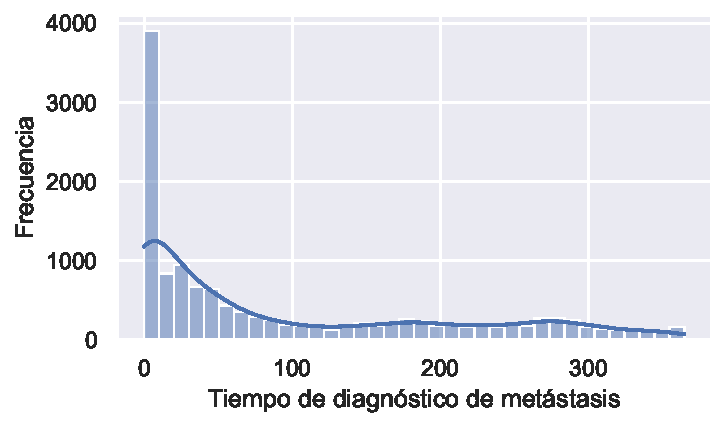
\includegraphics[width=\linewidth]{figs/chapter3/objectivevariable/diagnosisperioddistribution.pdf}
				\caption{Distribución general}\label{fig:ch3general}
			\end{center}
		\end{subfigure} 
		\begin{subfigure}{0.45\linewidth}
			\begin{center}
				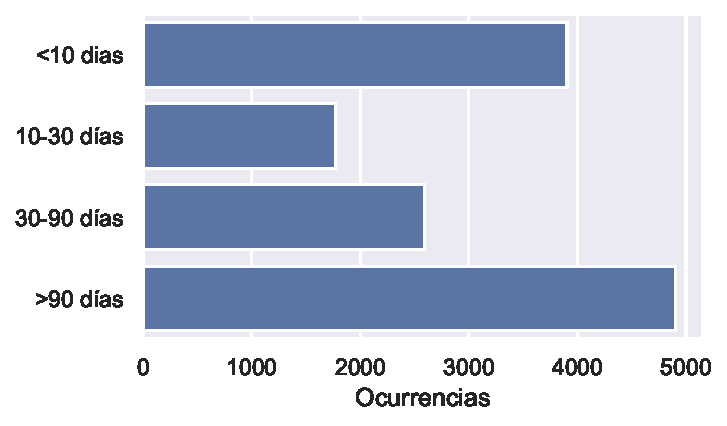
\includegraphics[width=\linewidth]{figs/chapter3/objectivevariable/diagnosisperiodgrouped.pdf}
				\caption{Distribución agrupada}\label{fig:ch3group}
			\end{center}
		\end{subfigure} 
	\end{center}
	\caption[Ejemplo de subfiguras]{Distribución del tiempo de diagnóstico}
	\label{fig:ch3varobjetivo}
\end{figure}

Se puede ver que los tiempos de diagnóstico siguen una \textbf{distribución de Poisson} - con la mayoría de casos diagnosticados en un rango de $[0-10]$ días. Ahora bien, como se observa en la \textbf{Figura \ref{fig:ch3group}}, si se agrupan los valores en rangos \textbf{la mayoría de casos tardan más de 90 días en ser diagnosticados}.

\subsubsection{Valores perdidos}

Antes de realizar un estudio más exhaustivo de los atributos, es de interés estudiar el comportamiento de los \textbf{valores perdidos} en el conjunto de datos - para comprobar si hay un gran número de éstos, si existen atributos irrelevantes por tener un alto grado de información perdida y si sería necesario realizar algún tipo de tratamiento sobre éstos valores.

\begin{figure}[h]
	\centering
	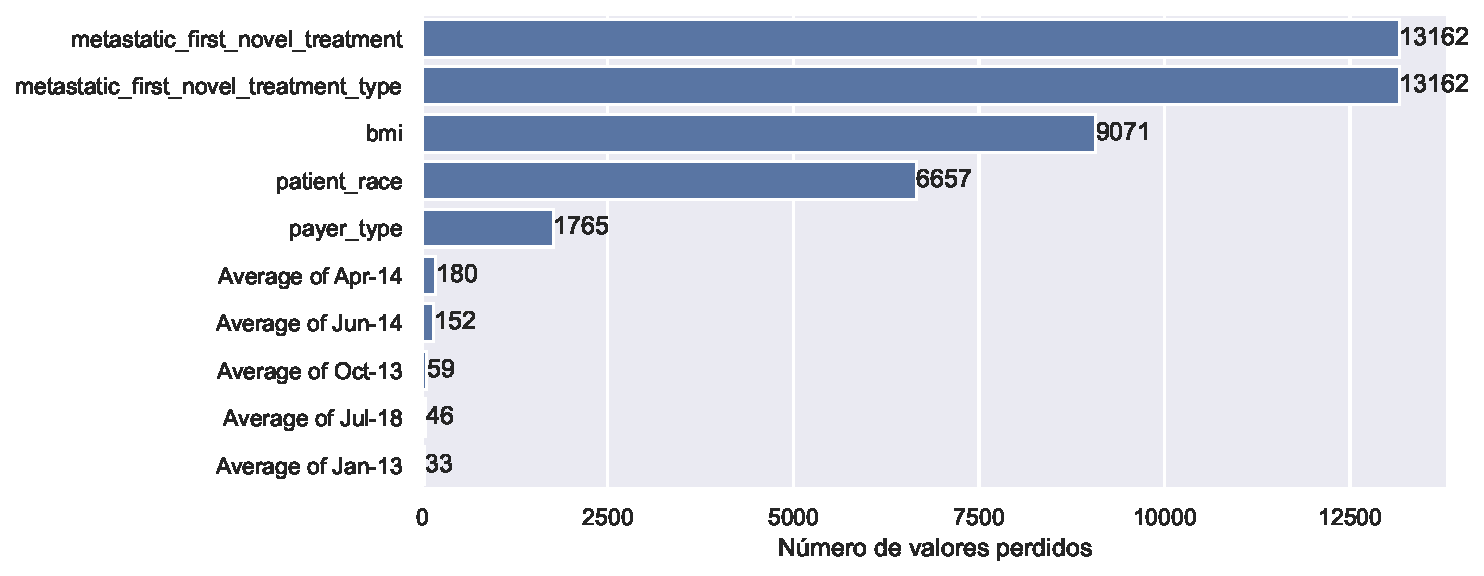
\includegraphics[width=0.9\linewidth]{figs/chapter3/missingvalues}
	\caption[Atributos con mayor número de valores perdidos]{Atributos con mayor número de valores perdidos}
	\label{fig:ch3missingvalues}
\end{figure}

Estudiando la distribución, \textbf{72} de los 150 atributos disponibles presentan valores perdidos - con un promedio de \textbf{624 instancias perdidas} por atributo. En primera instancia puede parecer un número muy elevado de valores perdidos, si se observa cómo se distribuyen los valores perdidos - como se representa en la \textbf{Figura \ref{fig:ch3missingvalues}} - se puede observar un \textbf{sesgo} claro, donde la amplia mayoría de valores perdidos se agrupan alrededor de cinco atributos:

\begin{itemize}
	\item \textbf{Tratamiento:} Debido al número tan elevado de valores perdidos en ambos atributos, \textbf{solo se tiene información sobre el tratamiento de 11 pacientes} - lo que significa que no sería relevante el atributo debido a la falta de información.
	\item \textbf{Índice de masa corporal del paciente:} Se conoce el índice de masa corporal de \textbf{menos de la mitad de los pacientes.}  Además, al ser información numérica \textbf{no existe un valor por defecto} por el que se puedan reemplazar los valores perdidos - por lo que sería razonable no estudiar en más detalle el atributo.
	\item \textbf{Raza y tipo de seguro médico del paciente:} En ambos casos hay un número considerable de instancias con valores desconocidos. Ahora bien y a diferencia del IMC, al ser atributos categóricos puede considerar que \textbf{es significativo para el estudio que no se conozcan estos valores} - tratándolos como una categoría adicional, \textit{"Desconocido"}.
\end{itemize}

En el resto de atributos el número de valores perdidos es más reducido - en el orden de \textbf{100 instancias} o menor -, por lo que el tratamiento es más simple, pudiendo descartar las instancias con valores perdidos o realizando una imputación simple con el valor promedio.

\subsection{Estudio de atributos categóricos}

\subsubsection{Datos personales - raza y género del paciente}

\subsubsection{Datos médicos - seguro, códigos de diagnóstico y tipos de tratamiento}

\subsubsection{Datos geográficos}

\subsection{Estudio de atributos numéricos}

\subsection{Conclusiones del análisis}